\subsection{\href{\linkengarts}{Engineered Arts}}
   \hypertarget{subsec:engineered_arts}
   Se desarrolló una placa de potencia y medición de corriente de gran precisión para un motor BLDC. Se tomaron los requisitos, se diseñó el esquemático, la selección de componentes y finalmente el ruteo del PCB como se ve en la figura \ref{fig:engineered_arts1}
     \begin{figure}
      \begin{center}
         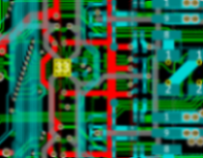
\includegraphics[width=0.3\textwidth]{engineered_arts1.png}
         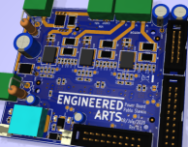
\includegraphics[width=0.3\textwidth]{engineered_arts2.png}
         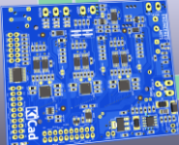
\includegraphics[width=0.3\textwidth]{engineered_arts3.png}
      \end{center}
      \caption{Placa electrónica PCB de potencia para medición y control de un motor BLDC para la empresa Engineered Arts \href \linkengartsrotbldc {ver placa en 3D}}
      \label{fig:engineered_arts1}
   \end{figure}
